%
% A Real Chapter
\chapter{Reinforcement Learning for Tracking Problem: A Survey} \label{chap::survey}
Despite the success of \ac{RL} in many robotics problem (e.g. learning to fly \cite{Abbeel}, walk \cite{NIPS2007_3253} and navigate \cite{4543641}), the application of \ac{RL} for tracking control is not a widely explored topic. Over the spans of the literature survey, author finds several attempts to exploits \ac{RL} for tracking problem, which can be categorized into 3 different approaches: dynamic tuning, \ac{RL} for optimal control, and \ac{RL} for nonlinear additive compensator. 

This chapter covers the foundational theory of the 3 aforementioned approaches. The main idea, advantages, limitations and ease of implementation are the key issues which will be discussed in the next chapter. These issues will serve as the basis of the argument to choose one method for later implementation. The chapter starts in Section \ref{sec:rl_lqt} by providing explanation about \ac{RL} for optimal tracking control. Section \ref{sec:dytun} deals with the so called dynamic tuning -- a class of gain scheduling which makes use of \ac{RL}. The third method, presented in Section \ref{sec:nl_comp}, is a relatively new approach which employs \ac{RL} to learn additive input compensation.


\section{Reinforcement Learning for Optimal Tracking Control} \label{sec:rl_lqt}
This method is initiated and developed by Lewis et. al. which aims to solve the tracking by \ac{RL} problem from dynamic programming perspective. The method uses optimal control, a branch of control theory whose root is closely related to dynamic programming \cite{126844}. The method starts from the downside of optimal tracking control which requires the solution of non-causal differential equation. It turns out that by assuming the reference to follow a certain dynamics and modifying the state of the optimal tracking, a causal representation can be obtained. Once a causality is in hand, we can then employ our favorite \ac{RL} techniques to asymptotically solve for the solution. 

To provide an easier comparison between the standard optimal tracking solution with \ac{RL}-based one, this section starts by formulating the standard optimal tracking problem and deriving its solution. Next, the modified formulation of optimal tracking which allows the causal formulation of infinite horizon optimal tracking problem is discussed. Following is the \ac{PI} algorithm to solve the optimal tracking. In this section, only discrete-time \ac{LQT} problem is considered \cite{Kiumarsi6760476}. Although the extension to non-linear and continuous time optimal tracking problem is not straightforward, the main steps are actually quite similar. The derivation presented in this section is based on work by Kiumarsi-Khomartash \cite{Kiumarsi6760476} with modifications to comply with the convention used in this report.

\subsection{Standard LQT problem}
The standard \ac {LQT} problem is treated extensively in \cite{lewis1995optimal}. First, we formulize the \ac {LTI} discrete-time system as 

\begin{equation} \label{eq:ss}
\begin{split}
x(k+1) &= Ax(k) + Bu(k) \\
y(k) &= Cx(k)
\end{split}
\end{equation}

where $x(j) \in \mathbb{R}^n$, $u(j) \in \mathbb{R}^m$ and $y(j) \in \mathbb{R}^l$ are the state, input and output at time instance $j$ respectively. While $A$, $B$, $C$ are the state matrices. For the sake of simplicity, we omit the feedthrough matrix $D$ and consider a \ac {SISO} system. The value of a certain state $x(k)$ and reference signal $r(k)$ can be formulized as the following infinite-horizon cost function

\begin{equation}
\label{eq:infcost}
J = V(x(k), r(k)) = \frac{1}{2} \sum_{i=k}^{\infty} (Cx(i)-r(i))^TQ(Cx(i)-r(i)) + u(i)^TRu(i)
\end{equation}

where $Q \geq 0$ and $R > 0$. The goal of LQT is to obtain the optimal tracking input $u^*(k)$ which minimizes $J$. This control input is given as a combination of feedback and feedforward term
\begin{equation}
u(k) = -Kx(k) + K_vv(k+1)
\end{equation}
where $v(k+1)$ can be obtained by solving a non-causal difference equation
\begin{equation}
v(k) = (A-BK)^Tv(k+1) + C^TQr(k)
\label{eq:noncausal}
\end{equation}
The control gains $K$ and $K_v$ are

\begin{equation}
K = (B^TSB + R)^{-1}B^TSA
\end{equation}

\begin{equation}
K_v = (B^TSB + R)^{-1}B^T
\end{equation}

where $S=S^T>0$ is a unique solution of the \ac {ARE} as follows

\begin{equation}
\begin{split}
S &= A^TS(A-BK) + C^TQC \\
&= A^TSA - A^TSB(B^TSB+R)^{-1}B^TSA + C^TQC
\end{split}
\end{equation}
Applying the optimal tracking input $u^*(k)$ gives us the minimal cost (optimal value) given by

\begin{equation}
J^* = V^*(x(k), r(k)) = \frac{1}{2}x(k)^TSx(k) - x(k)^Tv(k) + w(k)
\end{equation}

where $ w(k) $ is obtained from a backward recursion

\begin{equation}
w(k) = w(k+1) + \frac{1}{2}r(k)^TQr(k) - \frac{1}{2}v(k+1)^TB(B^TSB+R)^{-1}B^Tv(k+1)
\end{equation}

Clearly, the drawback of standard optimal tracking control is the necessity to solve a non-causal difference equation \eqref{eq:noncausal}. However, by assuming the reference trajectory to follow a certain dynamics, we can obtain a causal equation. This will be the subject of next subsection.

\subsection{Causal Representation of the LQT}
First, the necessary assumption is that the reference is generated by following stable difference equation
\begin{equation}
r(k+1) = Fr(k) 
\end{equation}
where $ F $ is hurwitz. By augmenting the state in \eqref{eq:ss}, we obtain the following new state space system

\begin{equation}
\begin{split}
\left[ \begin{array}{c}
x(k+1) \\ 
r(k+1)
\end{array} \right] &= \left[\begin{array}{cc}
A & \textbf{0} \\ 
\textbf{0} & F
\end{array}  \right] \left[ \begin{array}{c}
x(k) \\ 
r(k)
\end{array} \right] + \left[ \begin{array}{c}
B \\ 
\textbf{0}
\end{array} \right] u(k) \\
X(k+1) &= TX(k) + B_1u(k)
\end{split}
\end{equation}

Next, we assume that the candidate lyapunov function $V$ for the augmented state space system to be

\begin{equation}
\label{eq:lqtlyap}
V(x(k), r(k)) = V(X(k)) = \frac{1}{2}X(k)^TPX(k)
\end{equation}

where $ P = P^T > 0 $

Modifying the infinite-horizon cost function \eqref{eq:infcost}, we come up with a Bellman equation for LQT
\begin{equation}
\begin{split}
V(x(k), r(k)) = &\frac{1}{2} (Cx(k)-r(k))^TQ(Cx(k)-r(k)) + u(k)^TRu(k) + \\
&\frac{1}{2} \sum_{i=k+1}^{\infty} \left[ (Cx(i)-r(i))^TQ(Cx(i)-r(i)) + u(i)^TRu(i)\right] 
\end{split}
\end{equation}

\begin{equation}
\begin{split}
V(x(k), r(k)) = &\frac{1}{2} (Cx(k)-r(k))^TQ(Cx(k)-r(k)) + u(k)^TRu(k) + \\
& V(x(k+1), r(k+1))
\end{split}
\end{equation}

Inserting the lyapunov equation \eqref{eq:lqtlyap}, the LQT Bellman equation becomes
\begin{equation}
\label{eq:lqtbellman}
X(k)^TPX(k) =  X(k)^TQ_1X(k) + u(k)^TRu(k) + X(k+1)^TPX(k+1)
\end{equation}
where

\begin{equation}
Q_1 = \left[ \begin{array}{cc}
C^TQC & -C^TQ \\ 
-QC & Q
\end{array} \right] 
\end{equation}

From the LQT Bellman equation, one can compute the time derivative (skipped here) to obtain the LQT ARE.
\begin{equation}
\label{eq:lqtare}
Q_1 - P + T^TPT - T^TPB_1(R+B_1^TPB_1)^{-1}B_1^TPT = 0
\end{equation}

Solving for $P$ that satisfies \eqref{eq:lqtare}, we finally obtain the optimal policy 
\begin{equation}
\label{eq:opt_u}
u(k) = -K_1X(k)
\end{equation}
with
\begin{equation}
K_1 = (R+B_1^TPB_1)^{-1}B_1^TPT
\end{equation}
Our next objective is to compute $P$ of \eqref{eq:lqtare} in iterative manner using \ac {RL} instead of direct computation which might be unfeasible. 

\subsection{\ac{RL} for Solving the LQT ARE}
In this subsection, we will employ iterative learning algorithms to solve for $P$. Before that, we need to derive for the lyapunov equation from the LQT Bellman equation \eqref{eq:lqtbellman} by inserting the optimal \eqref{eq:opt_u}. This yields
\begin{equation*}
X(k)^TPX(k) =  X(k)^TQ_1X(k) + X(k)^TK_1^TRK_1X(k) + X(k)^T(T - B_1K_1)^TP(T - B_1K_1)X(k)
\end{equation*}
\begin{equation}
\label{eq:lyap_lqt}
\Leftrightarrow  P =  Q_1 + K_1^TRK_1 + (T - B_1K_1)^TP(T - B_1K_1)
\end{equation}

It turns out that by choosing a stabilizing initial policy $u^0 = -K_1^0X(k)$, one can use policy evaluation and iteration to approximate $ P $. In each iteration, the policy is guaranteed to be stable. The prove of this key theorem is given in \cite{1099755}. 

By taking this theorem, one can design both offline and online \ac{PI} algorithms to asymptotically approximate $P$. The offline \ac{PI} improves $P$ using the lyapunov function \eqref{eq:lyap_lqt}, while the LQT Bellman equation \eqref{eq:lqtbellman} is used for the online \ac{PI}. These two algorithms are listed in Algorithm~\ref{alg:off_pi} and \ref{alg:on_pi}. We can see that for the offline \ac{PI}, we can directly obtain $P$. Meanwhile, for the online \ac{PI}, $P$ needs to be solved with a least square method. Note that both require the knowledge of the system dynamics. If the model is not (fully) known, one can use Q-learning \cite{Kiumarsi20141167} or actor-critic \ac {RL} \cite{Modares20141780} instead. 

\begin{algorithm}[H]
	%	\KwData{this text}
	%	\KwResult{how to write algorithm with \LaTeX2e }
	\textbf{Initialization:} Select an admissible (stable) gain $K^0_1$\\
	\Repeat(){$ P $ converges}{
		\textbf{Policy evaluation:} \\
		$P^{j+1} = Q_1 + (K_1^j)^TRK_1^j + (T-B_1K_1^j)^TP^{j+1}(T-B_1K_1^j)$\\
		
		\textbf{Policy improvement:} \\
		$ K_1^{j+1} = (R+B_1^TP^{j+1}B_1)^{-1} B_1^TP^{j+1}T $\\	
	}
	\label{alg:off_pi}
	\caption{Offline Policy Iteration}
\end{algorithm}

\begin{algorithm}[H]
	%	\KwData{this text}
	%	\KwResult{how to write algorithm with \LaTeX2e }
	\textbf{Initialization:} Select an admissible (stable) gain $K^0_1$\\
	\Repeat{$ P $ converges}{
		\textbf{Policy evaluation:} \\
		$X(k)^TP^{j+1}X(k) = X(k)^T\left( Q_1 + (K_1^j)^TRK_1^j\right) X(k) + X(k+1)^TP^{j+1}X(k+1)$\\
		
		\textbf{Policy improvement:} \\
		$ K_1^{j+1} = (R+B_1^TP^{j+1}B_1)^{-1} B_1^TP^{j+1}T $\\	
	}
	\label{alg:on_pi}
	\caption{Online Policy Iteration}
\end{algorithm}

\subsection{\ac{RL} for \ac{LQT} with unknown system dynamics}
As the main goal of this thesis is to improve reference tracking by compensating for the unknown dynamics using \ac {RL}, the previously descibed \ac {PI} method which requires full information about the system dynamics is no longer relevant. In order to relax this requirement, we will turn to \ac {TD} learning. The solution to optimal tracking problem for a partially unknown system is given in \cite{Kiumarsi6760476} \cite{Kiumarsi6918527} and \cite{Modares20141780}. Although the method no longer requires drift dynamics $T$, input dynamics $B_1$ is still necessary. For a fully unknown system dynamics, a method proposed in \cite{Kiumarsi20141167} is the solution. 

We start by first defining the Q function as 
\begin{equation}
Q(X(k), u(k)) = \frac{1}{2}X(k)^TPX(k) 
\end{equation}
Then, multiplying \ac{LQT} Bellman equation \eqref{eq:lqtbellman} by $ \frac{1}{2} $ we obtain
\begin{equation}
\begin{split}
Q(X(k), u(k)) &= \frac{1}{2}X(k)^TQ_1X(k) + \frac{1}{2}u(k)^TRu(k) + \frac{1}{2}\gamma X^T(k+1)PX(k+1) \\
&= \frac{1}{2}X(k)^TQ_1X(k) + \frac{1}{2}u(k)^TRu(k) + \frac{1}{2}\gamma (TX(k) + B_1u(k))^TP(TX(k) + B_1u(k)) \\
&= \frac{1}{2}\left[  \begin{array}{c}
X(k) \\ 
u(k)
\end{array} \right] ^T \left[\begin{array}{cc}
Q_1+\gamma T^TPT & \gamma T^TPB_1 \\ 
\gamma B_1^TPT & R+\gamma B_1^TPB_1
\end{array}  \right] 
\left[  \begin{array}{c}
X(k) \\ 
u(k)
\end{array} \right] 
\end{split}
\label{eq:bellman_Q}
\end{equation}

Furthermore, we define the kernel matrix $H = H^T$ as
\begin{equation}
\begin{split}
H &=  \left[\begin{array}{cc}
Q_1+\gamma T^TPT & \gamma T^TPB_1 \\ 
\gamma B_1^TPT & R+\gamma B_1^TPB_1
\end{array}  \right] \\
&=\left[ \begin{array}{cc}
H_{XX} & H_{Xu} \\ 
H_{uX} & H_{uu}
\end{array} \right] 
\end{split}
\end{equation}
The the quadratic cost function reaches minimum when $ \frac{\partial Q(X(k), u(k))}{\partial u(k)} = 0 $. The input which satisfies this condition is
\begin{equation}
u(k) = -H_{uu}^{-1}H_{uX}X(k)
\end{equation}
Hence, by learning the value of $H$ online, we can obtain the optimal tracking input $u$ without the need of the system model. By modifying the infinite horizon cost function \eqref{eq:bellman_Q}, we write the Q function in Bellman equation format as

\begin{equation}
Q(X(k), u(k)) = \frac{1}{2}X(k)^TQ_1X(k) + \frac{1}{2}u(k)^TRu(k) + \gamma Q(X(k+1), u(k+1))
\label{eq:Bellman_Q2}
\end{equation}
Define $Z(k) = \left[ X(k)^T u(k)^T\right]^T$, the Q function can be written as
\begin{equation}
Q(X(k),u(k)) = \frac{1}{2}Z(k)^THZ(k)
\label{eq:Q_function}
\end{equation}
Combining equation~\eqref{eq:Bellman_Q2} with \eqref{eq:Q_function} yields
\begin{equation}
Z(k)^THZ(k) = X(k)^TQ_1X(k) + u(k)^TRu(k) + Z(k+1)^THZ(k+1)
\end{equation}

Finally, we can once again apply \ac {PI} to learn matrix $H$ online. This \ac {PI} is shown in Algorithm~\ref{alg:Q_pi}. Once again, $H$ can be calculated using a least square method after sufficient time instances.

\begin{algorithm}[H]
	%	\KwData{this text}
	%	\KwResult{how to write algorithm with \LaTeX2e }
	\textbf{Initialization:} Select an initial admissible (stable) control input $u = -K^0_1X_0$\\
	\Repeat{$ H $ converges}{
		\textbf{Policy evaluation:} \\
		$Z(k)^TH^{j+1}Z(k) = X(k)^TQ_1X(k) + (u(k)^j)^TRu(k)^j + Z(k+1)^THZ(k+1)$\\
		
		\textbf{Policy improvement:} \\
		$ u^{j+1}(k) = -(H_{uu}^{-1})^{j+1} H_{uX}^{j+1}X(k) $ 
	}
	\label{alg:Q_pi}
	\caption{Model-free Policy Iteration}
\end{algorithm}


\section{Dynamic Tuning via Reinforcement Learning} \label{sec:dytun}
In this second section, a class of method to improve tracking performance by dynamically tuned a controller's gain using \ac {RL} is presented. To the best of author's knowledge, there are two prominent methods which serve this purpose. The first method is relatively simple -- it starts from an admissible controller e.g. \ac{PID}, and tune the controller's gain according to the value function. The second method is a more complex approach which is based on a relatively new algorithm called \ac {PI$^2$}. It is a model-free, sampling based learning method derived from the principle of optimal control \cite{Buchli2010}. This algorithm has been shown to work for a variable impedance control \cite{Buchli6037312}, \cite{buchli2011learning}, \cite{theodorou2010generalized} to enable a manipulator performing task like flipping a light switch \cite{buchli2011learning}.

\subsection{Direct Tuning of Nominal Controller}
In many cases of reference tracking, a linear controller such as \ac{PID} only performs well for a certain condition (e.g. a particular reference signal and a region of state) in which the gain is tuned. For different conditions, the performance is most likely degraded or even worse, the response becomes unstable. Intuitively, one would call for a solution which adjusts the controller gain with respect to the current condition. This method, also known as gain scheduling, has been developed for quite some time. The most common techniques used are fuzzy logic \cite{375142} \cite{5229855} \cite{1684589} and neural networks \cite{6606304} \cite{572744} \cite{556252}. The main drawback of the two methods, however, lies on the scheduling mechanism which must be predefined. For instance with fuzzy logic, we need to define the fuzzy rules for the gain scheduling. For a system with a large number of states or a \ac {MIMO} system, this could become a tedious task. For such cases, it is interesting to use \ac {RL} to achieve an online gain scheduling. Surprisingly, the online gain scheduling by using \ac {RL} is not a widely explored topic. \cite{882916} and \cite{Brujeni5669655} serve as relevant examples out of few search results.

In this literature report, author will refer to the work by Brujeni et. al. \cite{Brujeni5669655}. Although the paper's application is about chemical process, the technique presented is still considered suitable for robotics. The simplified block diagram of this method is shown in Figure~\ref{fig:dynamictuning}. As the figure depicts, the idea of dynamic tuning is pretty general thus can be extended to a number of \ac {RL} algorithms (e.g. actor critic, Q-learning) and controllers. However, in order to present a more concrete example, we will explain a specific method used in the paper -- a class of \ac {TD} learning called \ac{SARSA} with \ac{PID} controller. 

\begin{figure}[h!]
	\centering
	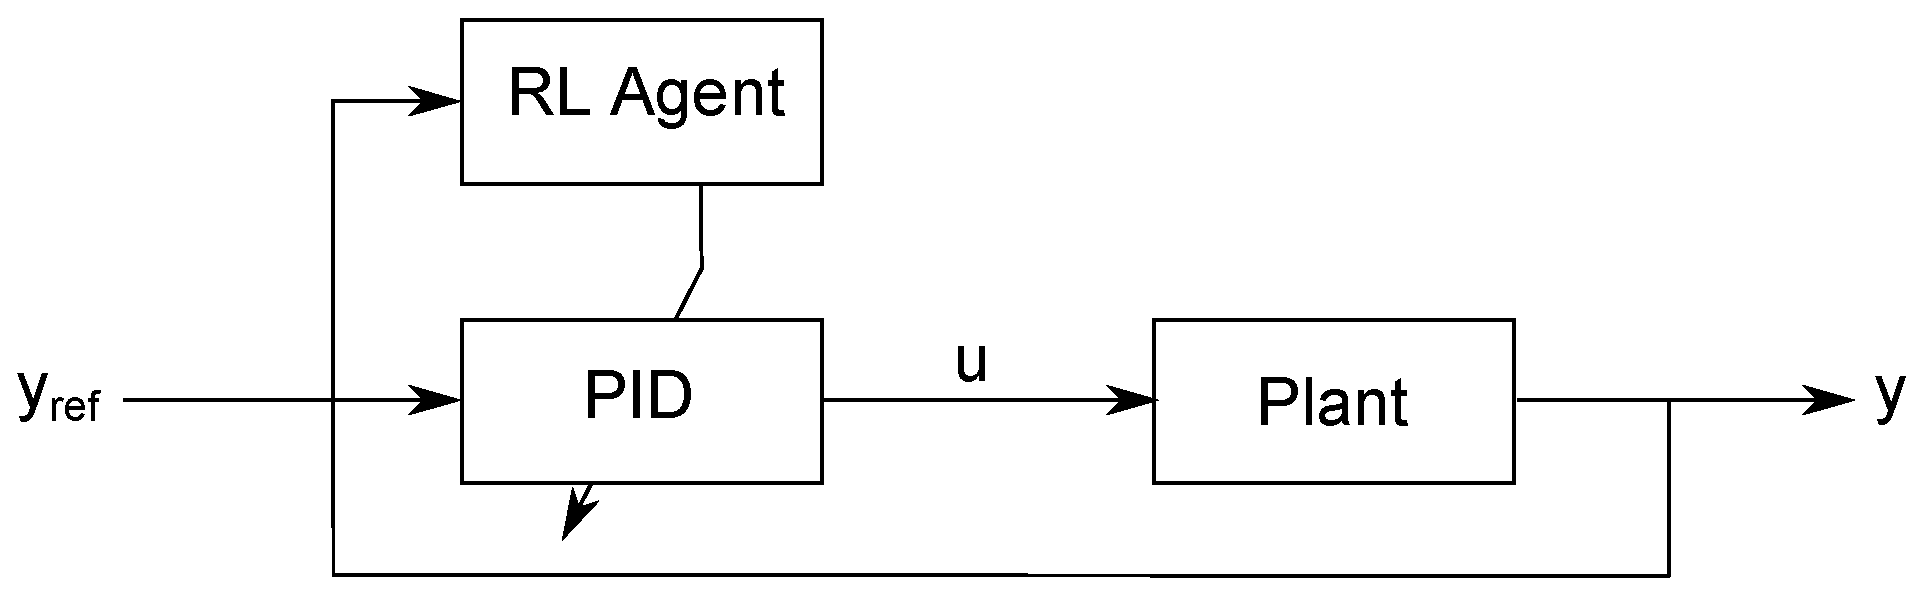
\includegraphics[width=0.7\linewidth]{dynamictuning}
	\caption{Gain scheduling of Nominal controller using \ac {RL}. In this case, a \ac{PID} controller is used}
	\label{fig:dynamictuning}
\end{figure}

	\subsubsection{\ac{SARSA} algorithm} 
	Consider a sequence of state and action as depicted in Figure~\ref{fig:sarsa}. We start by applying control signal $ u(k) $ at an initial state $ x(k) $, yielding a reward $ r(k+1) $ and the next state $ x(k+1)$. Following the same policy $\pi$, we apply the next action $ u(k+1) $, hence the name \ac {SARSA}. One of the objective is to learn the action-value function $ Q^{\pi}(x,u) $ while following a fixed policy $ \pi $ over an episode. The pseudo-code of \ac{SARSA} is given in Algorithm~\ref{alg:sarsa} where $ \alpha, \gamma \in [0 \dots 1]$ and $r$ are learning rate, discount rate and immediate reward respectively \cite{sutton1998reinforcement}. Note that instead of updating $Q$ by taking the optimal action at next step, \ac {SARSA} sticks to the action resulting from the policy $\pi$ (see line 8 of the algorithm). Therefore, \ac {SARSA} is a type of on-policy \ac {RL} algorithm.
	
	
	\begin{figure}[h!]
		\centering
		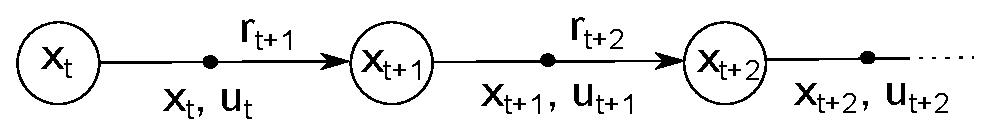
\includegraphics[width=0.7\linewidth]{sarsa}
		\caption{A sequence of state and action}
		\label{fig:sarsa}
	\end{figure}
	
	\begin{algorithm}[H]
		%	\KwData{this text}
		%	\KwResult{how to write algorithm with \LaTeX2e }
		\textbf{Initialization:} Initialize $ Q(x,u) $ arbitrarily\\
		\Repeat( for each episode:){episodes run out}{
			Initialize $ x $ \\
			Choose $ u $ from $ x $ using policy derived from $ Q $ \\
			\Repeat ( for each step of episode:){s is terminal}{
				Take action $ u $, observe $ r $, $ x' $ \\
				Choose $ u' $ from $ x' $ using policy derived from $ Q $ \\
				$ Q(x,u) \leftarrow Q(x,u) + \alpha[r+\gamma Q(x',u')-Q(x,u)] $	\\
				$ x \leftarrow  x' $\\
				$ u \leftarrow  u' $
			}
		} 		
		\label{alg:sarsa}
		\caption{SARSA algorithm}
	\end{algorithm}
	
	\subsubsection{\ac{SARSA} + \ac{PID} controller}
	To incorporate \ac{SARSA} for gain scheduling purpose, we define the policy $\pi$ as the gain modifier (see Figure~\ref{fig:dynamictuning}) instead of control input generator. In other words, $\pi$ will return the controller parameters e.g. $ K_p $ $ K_i $ and $ K_d $ gains for \ac{PID} controller. In each iteration $\pi$ will be improved by observing the most-updated value function $Q$. Furthermore, the performance of the \ac {RL}-tuned controller needs to be evaluated in every $ N $-steps to see if the method is actually improving the tracking performance. One possible measure for evaluation is the \ac {ISE}
	\begin{equation}
	ISE = \sum_{k=0}^{N}e(k)^2 = \sum_{k=0}^{N}(y_d(k) - y_m(k))^T(y_d(k) - y_m(k))
	\end{equation}
	where $y_d$ and $y_m$ denotes desired and measured output respectively. It is also suggested to evaluate the value at each time step $Q(x(k), u(k))$. A more concrete example of a \ac{PID} controller for a linear discrete time system is presented in Algorithm~\ref{alg:pid_sarsa}.
	
	\begin{algorithm}[h]
		%	\KwData{this text}
		%	\KwResult{how to write algorithm with \LaTeX2e }
		\textbf{Initialization:} Initialize $ Q $\\
		\For{j = 1 to $ N_{episode} $}{
			Initialize $ x_0 $ \\
			\For{$ k=0 $ to $ N_{steps}-1 $}{
				\vspace{5mm}
				\textit{Compute \ac{PID} gains, error, and control input} \\
				$ K_p, K_i, K_d = \pi(x(k)) $ \\
				$ e(k) = y_d(k) - y_m(k) $ \\
				$ u(k) = K_pe(k) + K_i\sum_{i=0}^{k}e(k) + K_d[e(k)-e(k-1)]  $\\
				\vspace{5mm}		
				\textit{Update state and output} \\
				$ x(k+1) = Ax(k) + Bu(k) $\\
				$ y(k+1) = Cx(k+1) + Du(k+1) $\\				
				\vspace{5mm}
				\textit{Compute immediate reward} \\
				$ r(k+1) = \rho(x(k), u(k)) = \rho(x(k+1)) $ \\			
				\vspace{5mm}
				\textit{Compute \ac{PID} gains, error, and control input for the next time instance} \\
				$ K_p, K_i, K_d = \pi(x(k+1)) $ \\
				$ e(k+1) = y_d(k+1) - y_m(k+1) $ \\
				$ u(k+1) = K_pe(k+1) + K_i\sum_{i=0}^{k}e(k+1) + K_d[e(k+1)-e(k)]  $ \\
				\vspace{5mm}
				\textit{Update value functio}n \\
				$ Q(x(k), u(k)) \leftarrow Q(x(k), u(k)) + \alpha[r(k+1)+\gamma Q(x(k+1), u(k+1))-Q(x(k), u(k))] $	\\
				\vspace{5mm}
				modify $ \pi $ based on $ Q(x(k), u(k)) $
			}								
		}						
		\caption{\ac{PID} gain scheduling with \ac {SARSA}}
		\label{alg:pid_sarsa}
	\end{algorithm}
	

\subsection{Gain scheduling with \ac{PI$^2$}}
The second method of dynamic tuning is inspired by the sophisticated motor control of living animals. Biological motor control has shown superiority in terms of versatility and robustness to adapt to different task scenarios. Researchers have been trying to transfer the same capability to robots through variable impedance control. This task requires gain scheduling which, in one way, can be achieved by \ac{PI$^2$} algorithm. One of the main advantage of \ac{PI$^2$} is the scalability for robots with high \ac {DoF}. Although variable impedance control is the only application of \ac{PI$^2$} for robotics so far \cite{Buchli2010}, \cite{Buchli6037312}, \cite{buchli2011learning}, the method seems to be suitable for tracking application as well. Before moving on the motivation of such argument, we will summarize the \ac{PI$^2$} algorithm and its application for variable impedance control first.    

Let a continuous-time (non)linear dynamics described as 
\begin{equation}
\dot{x_t} = f(x_t) + G(x_t)(u_t + \epsilon_t)
\end{equation}
where $ G(x_t) \in \mathbb{R}^{n \times m }$ is the control matrix and $ \epsilon_t  \sim (0, \Sigma_{\epsilon}) $ is a zero-mean random variable. The key prerequisite before applying \ac{PI$^2$} is to transform the model-based stochastic optimal control problem into an approximation path integral problem. The goal of stochastic optimal control is to find an optimal input which minimizes a finite horizon cost function

\begin{equation}
J_{t_i} = V(X_{t_i}) = \underset{u_{t_i:t_N}}{\text{min}} e_{\tau_i}[R(\tau_i)]
\end{equation}
with 
\begin{equation}
R(\tau_i) = \phi_{t_N} + \int_{t_i}^{t_N}r_t dt
\end{equation}
where $ \phi_{t_N} $ is the terminal reward received at time $ t_N $ and $ \tau_i $ is a trajectory starts at time $ t_i $ and finishes at time $ t_N $. The immediate reward can be formulized as
\begin{equation}
r_t = r(x_t, u_t) = q_t + \frac{1}{2}u_t^TRu_t
\end{equation}

with $R>0$ and $q_t = q(x_t) $ is an arbitrarily chosen function, providing a degree of freedom in specifying the cost. Next, we derive the \ac {HJB} equation according to  \cite{stengel1994}

\begin{equation}
\partial _tV_t = q_t + (\partial _xV_t)^Tf(x_t)-\frac{1}{2}(\partial _xV_t)^TG_tR^{-1}G_t^T(\partial _xV_t) + \frac{1}{2}trace((\partial _{xx}V_t)G_t\Sigma_{\epsilon}G_t^T)
\end{equation}

where $ \partial _x $ and $ \partial _{xx} $ denotes jacobian and hessian respectively. Furthermore, we introduce assumptions that value function can be transformed into a logarithmic function $V_t = -\lambda$log$\Psi_t$ and $\lambda G_tR^{-1}G_t^T = G_t\Sigma_{\epsilon}G_t^T = \Sigma(x_t) = \Sigma_t$, which give us
\begin{equation}
-\partial _t\Psi_t = -\frac{1}{\lambda}q_t\Psi_t+ f(x_t)^T(\partial _x\Psi_t) + \frac{1}{2}trace((\partial _{xx}V_t)G_t\Sigma_{\epsilon}G_t^T)
\label{eq:kolmo_pde}
\end{equation}
In order to solve the so called Kolmogorov backward \ac {PDE} \eqref{eq:kolmo_pde}, we need to use Feynman Kac formula which provides a numerical approximation of the solution. The detailed derivation can be seen in \cite{oksendal2010} and \cite{5509336}. The solution of \eqref{eq:kolmo_pde} becomes
\begin{equation}
\Psi_{t_i} =  \underset{dt \leftarrow 0}{\text{lim}} \int p(\tau_i|x_i)exp \left[ -\frac{1}{\lambda}\left( \psi_{t_N} + \sum\limits_{j=0}^{N-1}q_{t_j}dt\right)\right] d\tau_i 
\label{eq:pathintegral} 
\end{equation}
Equation~\eqref{eq:pathintegral} is called path integral problem. The optimal control input can be derived:

\begin{equation}
\begin{split}
u_{t_i} &= \int P(\tau_i) u(\tau_i) d\tau_i \\
u(\tau_i) &= R^{-1}G_{t_i}^T(G_{t_i}R^{-1}G_{t_i}^T)^{-1}(G_{t_i}\epsilon_{t_i}-b_{t_i}) 
\end{split}
\end{equation}

with $P(\tau_i)$ is the probability of trajectory $\tau_i$ and $b_{t_i}$ is a complex notation which is explained in \cite{5509336}. This concludes the problem formulation for the stochastic optimal control.

It turns out that the \ac{PI$^2$} algorithm can be casted into the stochastic optimal control problem with parameterized control policy expressed as follows
\begin{equation}
a_t = g_t^T(\theta+\epsilon_t)
\end{equation}
One of the example of trajectory generator with parameterized policy is \ac {DMP} \cite{ijspeert2002learning}. The \ac{DMP} generates desired trajectory with a point of attractor $g$ and initial state $q_0$. The dynamics of \ac {DMP} is given as follows
\begin{align}
\frac{1}{\tau} \dot{v}_t &= f_t + g^T_t(\theta+\epsilon_t) \\
\frac{1}{\tau} \dot{q}_{d,t} &= v_t \\
f_t &= \alpha(\beta(g-q_{d,t})-v_t)\\
\frac{1}{\tau}\dot{s}_t &= -\alpha s_t\\
[g_t]_j &= \frac{w_js_t}{\sum_{k=1}^{p}w_k}(g-q_0)\\
w_j &= \text{exp}(-0.5h_j(s_t-c_j)^2)\\
\end{align}

The \ac{PI$^2$} algorithm will learn the optimal parameter $\theta$ which yields the optimal smooth trajectory so that the robot will go through a via-point $g$. The particular applications of such behavior are to enable robots performing task like swinging, catching, etc. The simulation and practical results presented on \cite{Buchli2010} and \cite{Buchli6037312} provide an example of an intermediate goal $g$ which the robot initially can not reach. After a number of iterations, the \ac{PI$^2$} algorithms finally manages to generate the optimal trajectory which enables to robot to reach $g$. The results also shows that \ac{PI$^2$} performs superior compared to standard \ac {RL} algorithms. This property of \ac{PI$^2$} with \ac {DMP} is interesting for tracking application if the points of attractor could be extended to a complete trajectory. To the best of author's knowledge, there is still no paper which gives the application reference tracking. Therefore, this method is one of the possible solutions for the thesis problem.

\section{Nonlinear Input Compensation via Reinforcement Learning} \label{sec:nl_comp}
The third method is a relatively new solution originated from \ac {DCSC}. As the name suggested, the idea is to learn an additive compensator to the reference signal by means of \ac{RL}. The proposed method is slightly different from the one presented in \cite{Efe2014} in the sense that the compensator is added directly to the reference signal $q_{ref}$ instead of the controller output $ u $. Furthermore, we specifically choose standard actor-critic \ac{RL} instead of \ac{MLAC} since we are not interested in learning the system model online for the sake of safety. The simplified block diagram of the control scheme is shown in Figure~\ref{fig:blockdiagram}. 

\subsection{Actor-critic formulation}
First, we need to parameterize the actor and critic using \ac {LLR} approximation \cite{Grondman6096441}. The actor and critic becomes $\pi(x_k,\vartheta_{k-1})$ and $V(x_k,\theta_k)$ respectively. As previously explained in Algorithm~\ref{alg:actorcritic}, the actor-critic will update the parameters $\theta$ and $\vartheta$ at each iteration. The fact that it uses partial derivative of value function makes actor-critic belongs to the so called policy gradient methods. Secondly, we propose the cost function as
\begin{equation}
r_k = \rho(y_m(k), y_d(k), u(k)) = (y_d(k) - y_m(k))^TQ(y_d(k) - y_m(k)) + u(k)^TRu(k)
\end{equation}
with $ Q \geq 0 $ and $ R>0 $ which is similar to that of \ac {LQT}. The possibility for a different cost function is very likely since choosing the suitable cost function itself is not a trivial problem.


\begin{figure}[h]
	\centering
	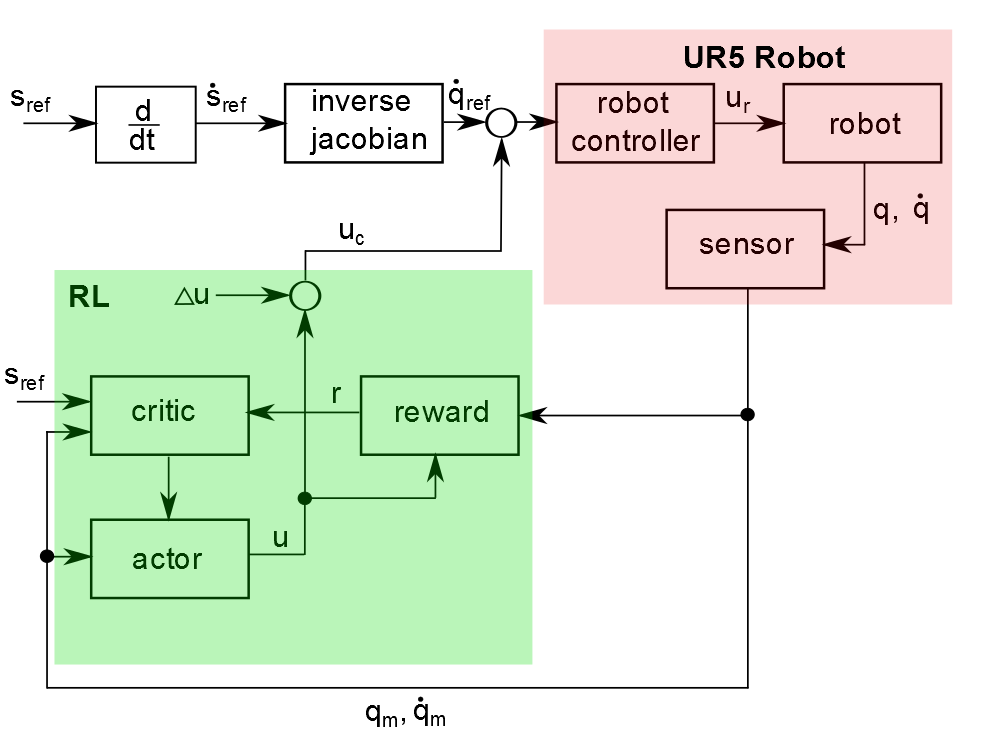
\includegraphics[width=0.7\linewidth]{blockdiagram}
	\caption{Block diagram of robot with \ac{RL} block acting as an additive compensator}
	\label{fig:blockdiagram}
\end{figure}

\subsection{\ac{LLR} Function Approximator}
The function approximator is needed since we are dealing with continuous state space. Popular examples of function approximator include fuzzy \cite{Efe2014}, neural networks \cite{Kiumarsi6918527} and \ac {LLR} \cite{Grondman6096441}. In this literature study, we will consider the latter due to its relatively simple and intuitive algorithm compared those of, for instance, neural network. The idea of \ac {LLR} is to approximate a non-linear function by predicting an output $\hat{y}_q$ to a certain query $x_q$ through a local fitting. This local fitting is performed by means of linear regression with respect to points $X$ which are close to $x_q$.  
The measure of distance is done by assigning weights into each point $x_i$ in the data base. 

A sorting algorithm can be employed to select $K$ number of closest neighbors from the database. Once these neighbor samples are selected, the input and output samples are said to be related with a simple linear function

\begin{equation}
Y = \beta X
\end{equation}

where 

\begin{equation}
\begin{split}
Y = \left[ \begin{array}{cccc}
y_1 & y_2 & \dots & y_K
\end{array} \right] \\
X = \left[ \begin{array}{cccc}
x_1 & x_2 & \dots & x_K \\ 
1 & 1 & \dots & 1
\end{array}  \right] 
\end{split}
\end{equation}
with the last row of $X$ is meant for bias term. The parameter $\beta$ is then computed using pseudo-inverse
\begin{equation}
\beta = YX^T(XX^T)^{-1}
\end{equation}
Now the predicted output $y_q$ can be calculated as
\begin{equation}
\hat{y}_q = \beta x_q
\end{equation}
The more samples in $X$ and $Y$, in other words the denser the neighborhood, the more accurate the prediction would be.



%\section{Iterative Learning Control} \label{sec:ilc}
%This is third section.

%\subsection{Case Study: 1-DOF Robot Gravity Compensation}

